\begin{figure}
    \centering
    \setlength{\resLen}{0.8in}
    \addtolength{\tabcolsep}{-3pt}
    \begin{tabular}{cccc}
        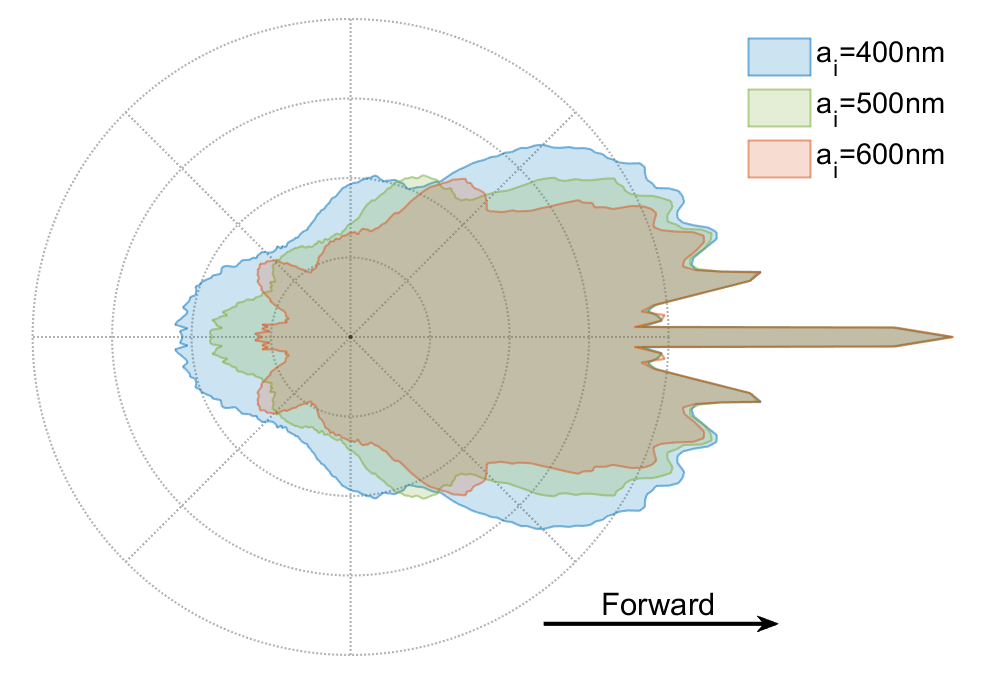
\includegraphics[width=\resLen]{images/pfunc/radius.png} &
        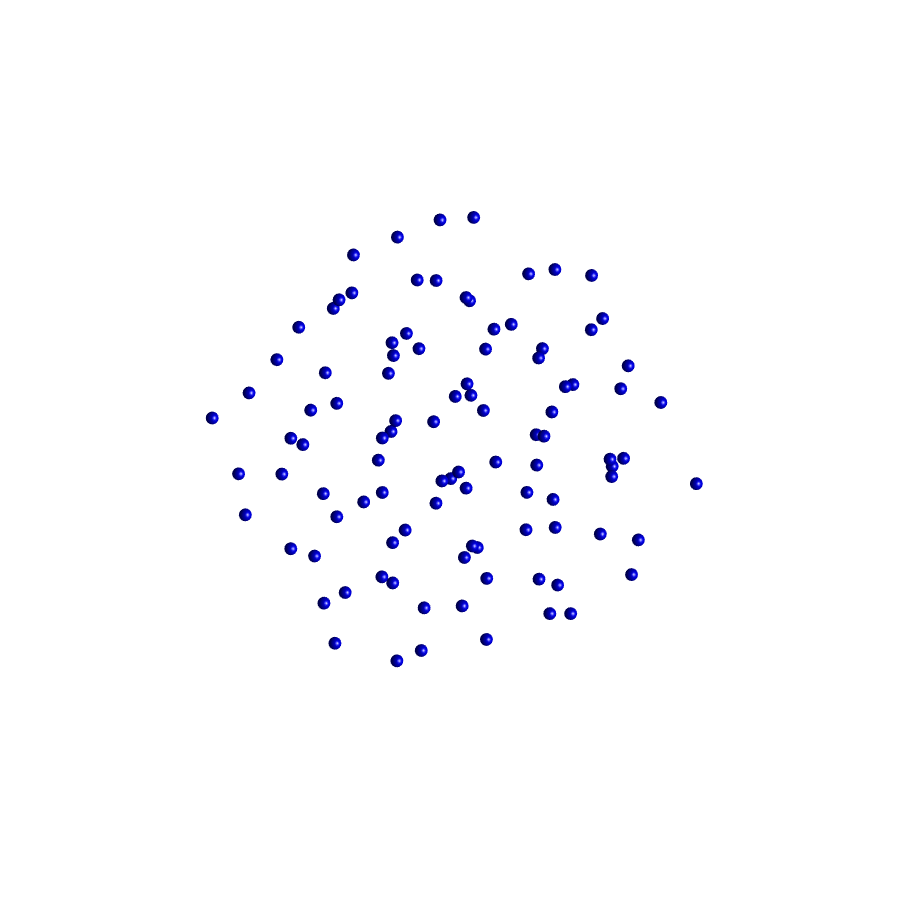
\includegraphics[width=\resLen]{images/particle/validate5_D2_N100_400nm.png} &
        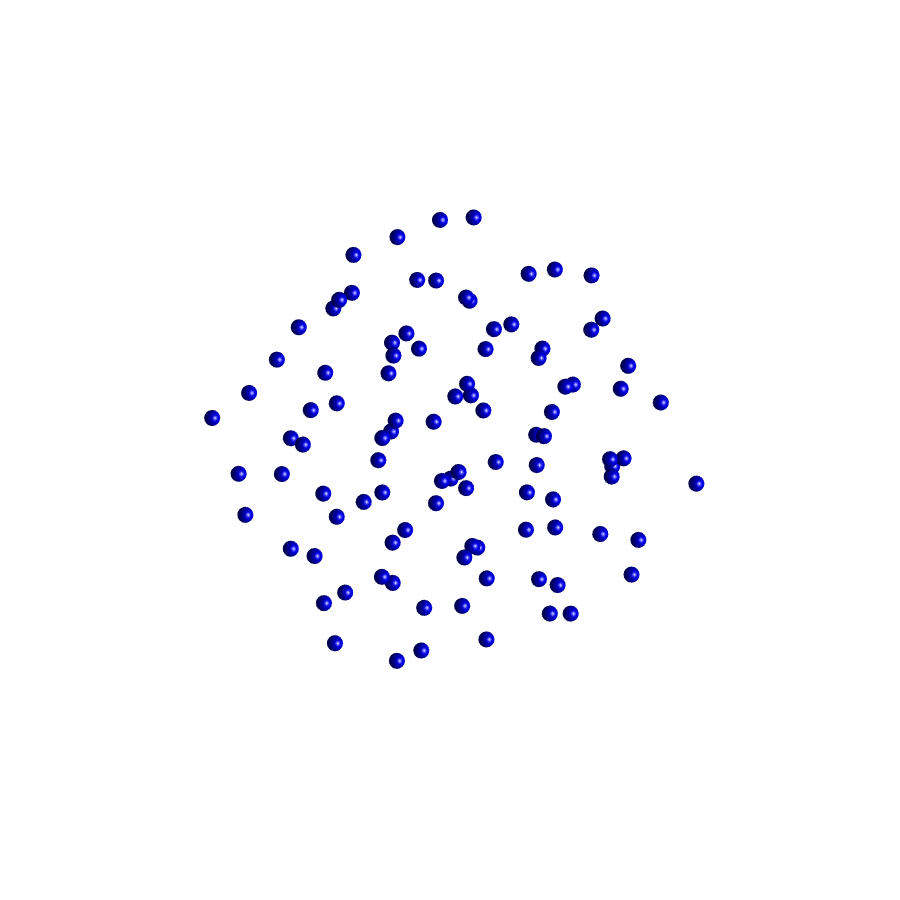
\includegraphics[width=\resLen]{images/particle/validate3_D2_N100_500nm.png} &
        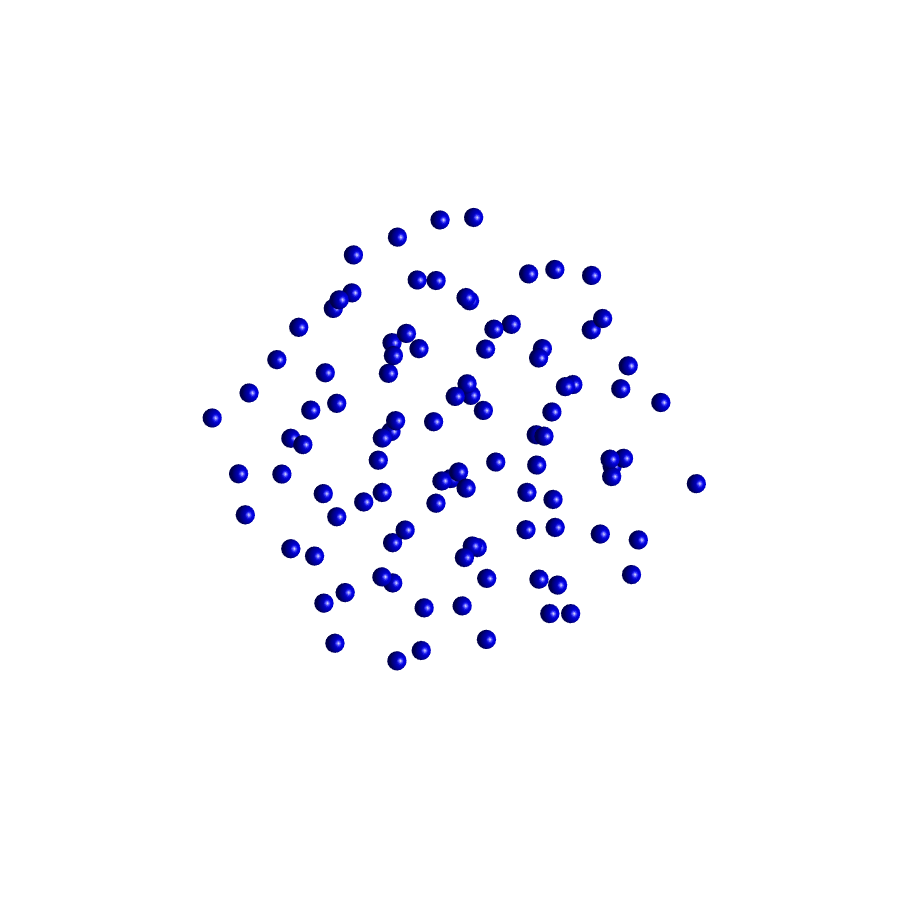
\includegraphics[width=\resLen]{images/particle/validate7_D2_N100_600nm.png} 
        \\ 
        Phase function & r=400nm & r=500nm & r=600nm
    \end{tabular}
    \caption{\label{fig:paritclesize}
        Different particle size. Wavelength is 700nm, and 100 particles in a cluster.
    }
\end{figure}

